\documentclass{eceday}

\graphicspath{{./Images/}}
\addbibresource{../References.bib}

\title[Chipyard]{Chipyard: A RISC-V Development Framework}
\subtitle{ECE Day 2021}
\author{Alexander Lukens \and Karl Hallsby}
\institute{Illinois Institute of Technology}
\date{\DTMdisplaydate{2021}{4}{9}{-1}}

\begin{document}

\nocite{chipyard}

\begin{frame}
  \titlepage{}
\end{frame}

\section{About Us}\label{sec:About_Us}
\begin{frame}
  \frametitle{\nameref{sec:About_Us}}
  
  \begin{columns}
    % Alex Picture and Description
    \begin{column}{0.50\linewidth}
      \begin{figure}[h!tbp]
        \centering
        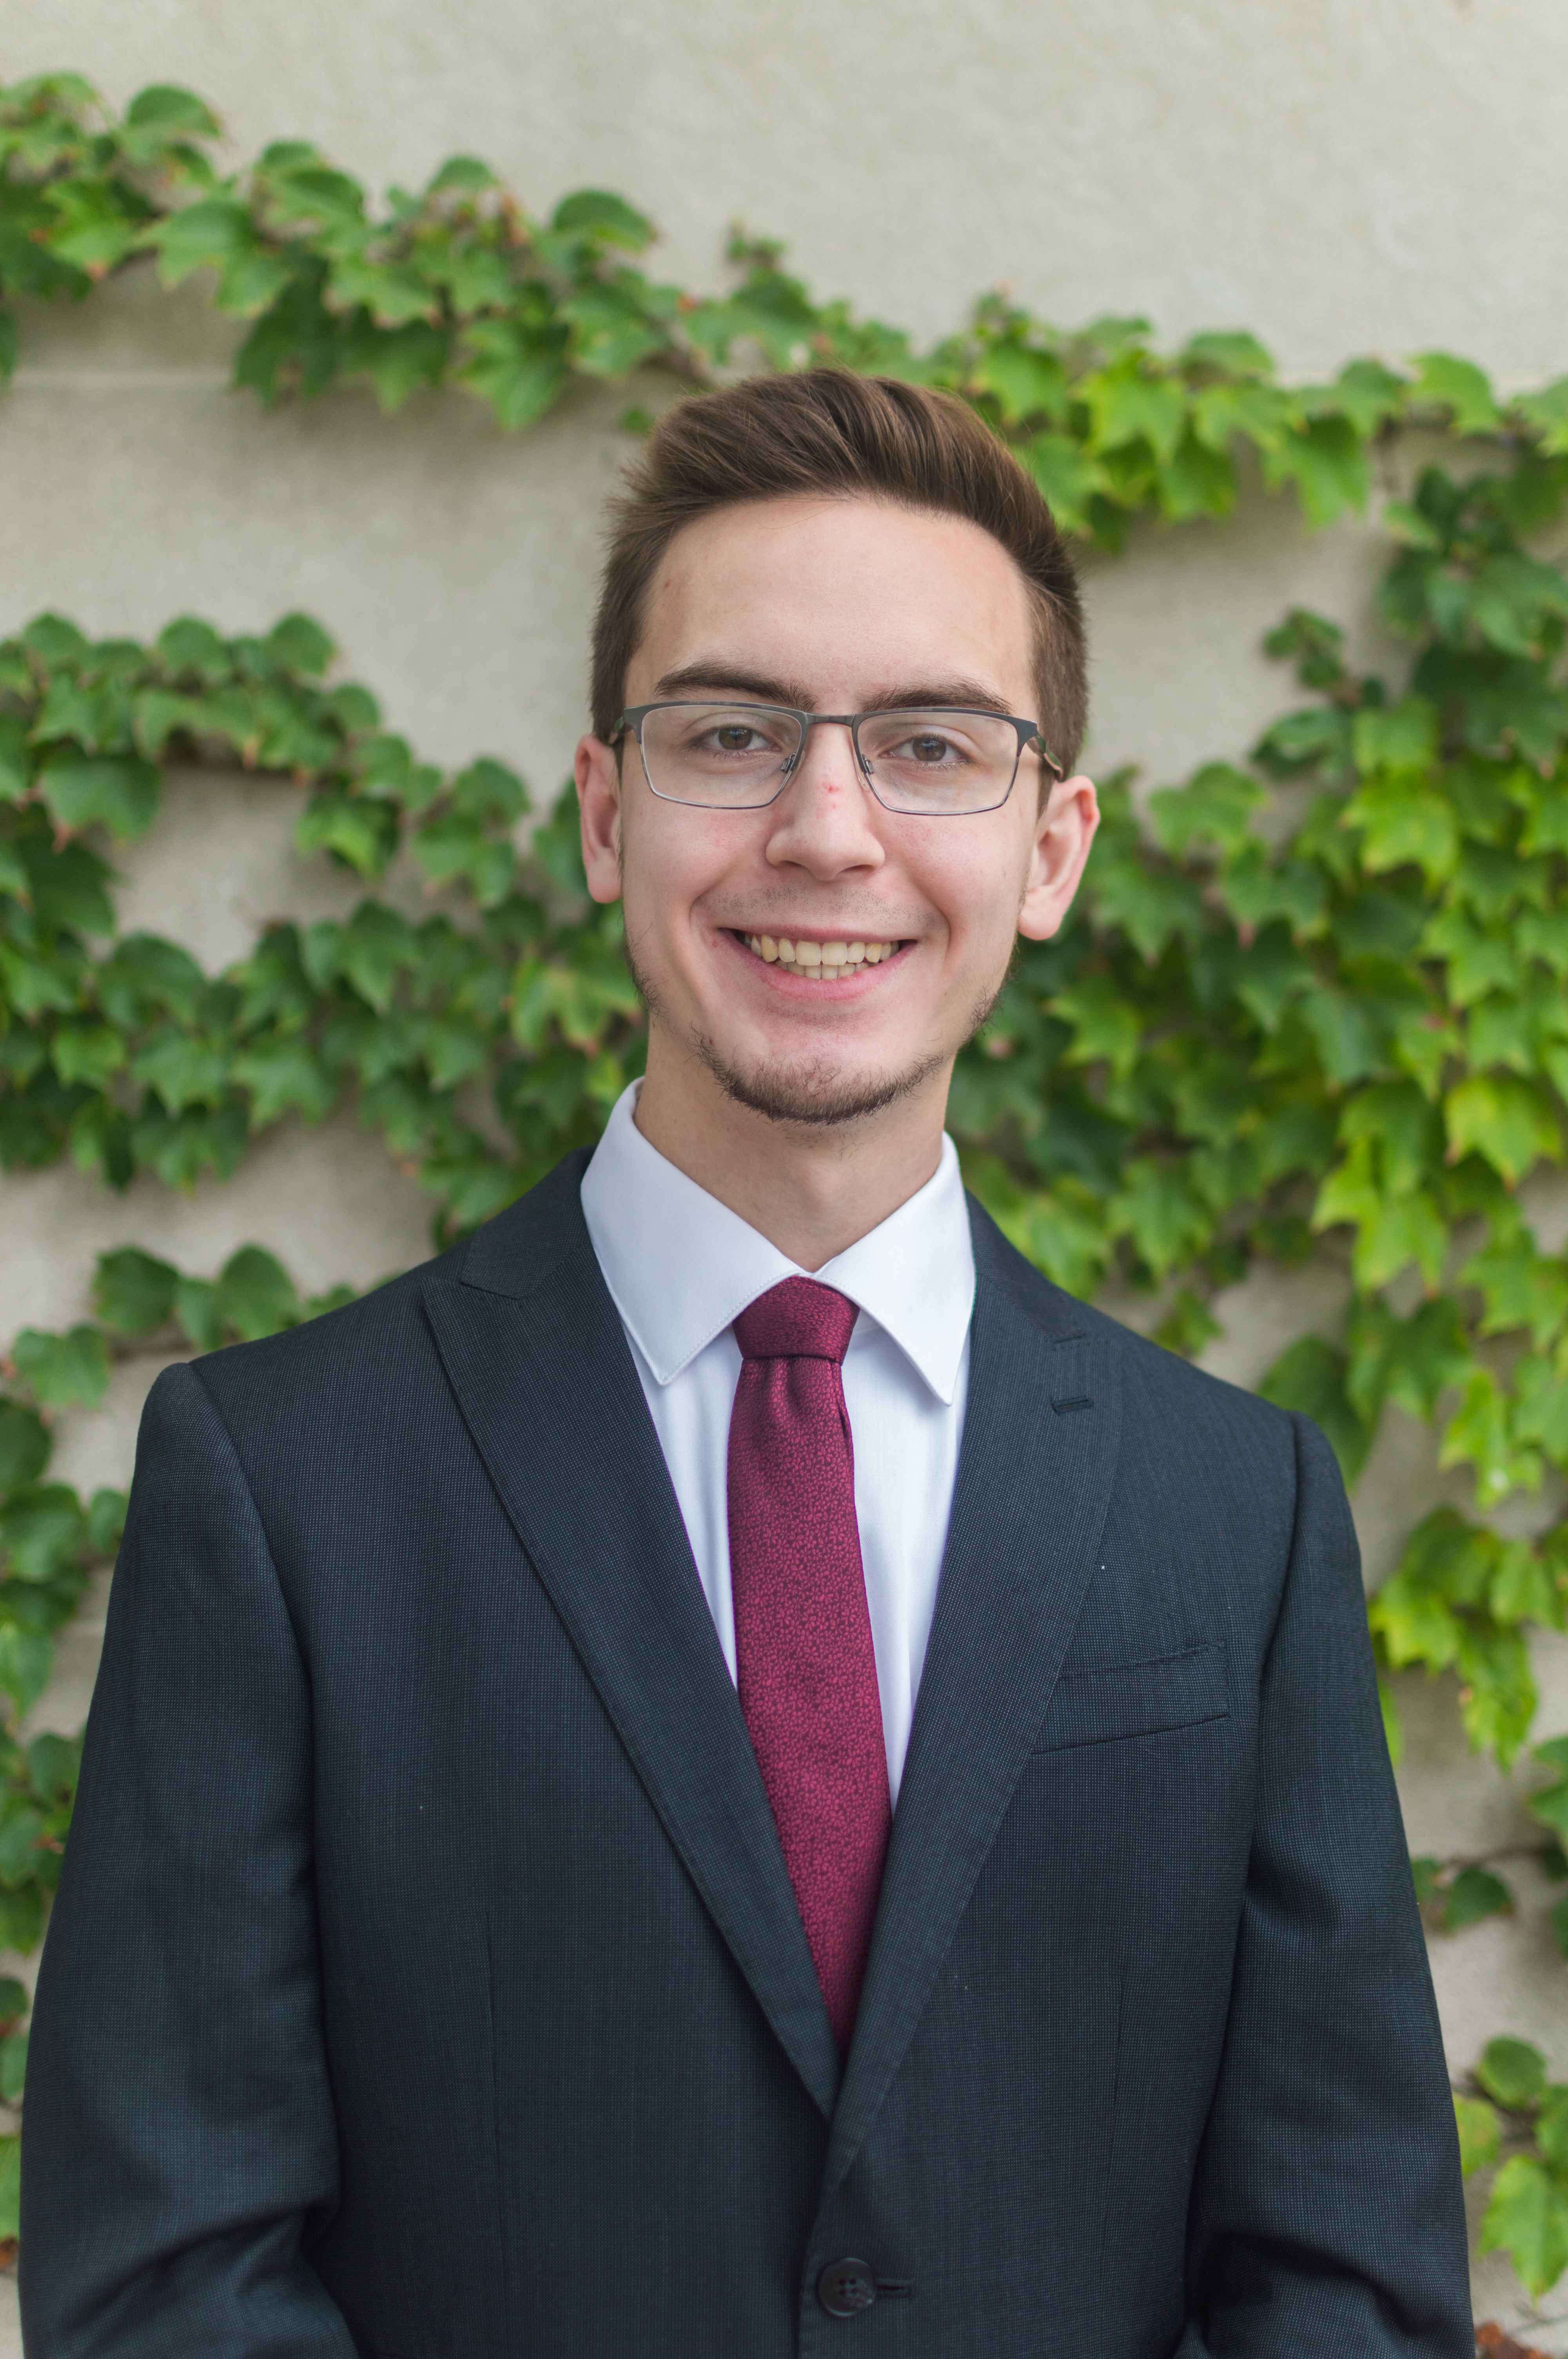
\includegraphics[scale=0.02]{./Lukens_Alex.jpg}
        \caption*{Alexander Lukens}
        \label{fig:Alex_Lukens}
      \end{figure}
  		\begin{centering}
  			B.S. Electrical Engineering
  			\newline M.S. Computer Engineering
  		\end{centering}

    \end{column}
    % Karl Picture and Description
    \begin{column}{0.50\linewidth}
      \begin{figure}[h!tbp]
        \centering
        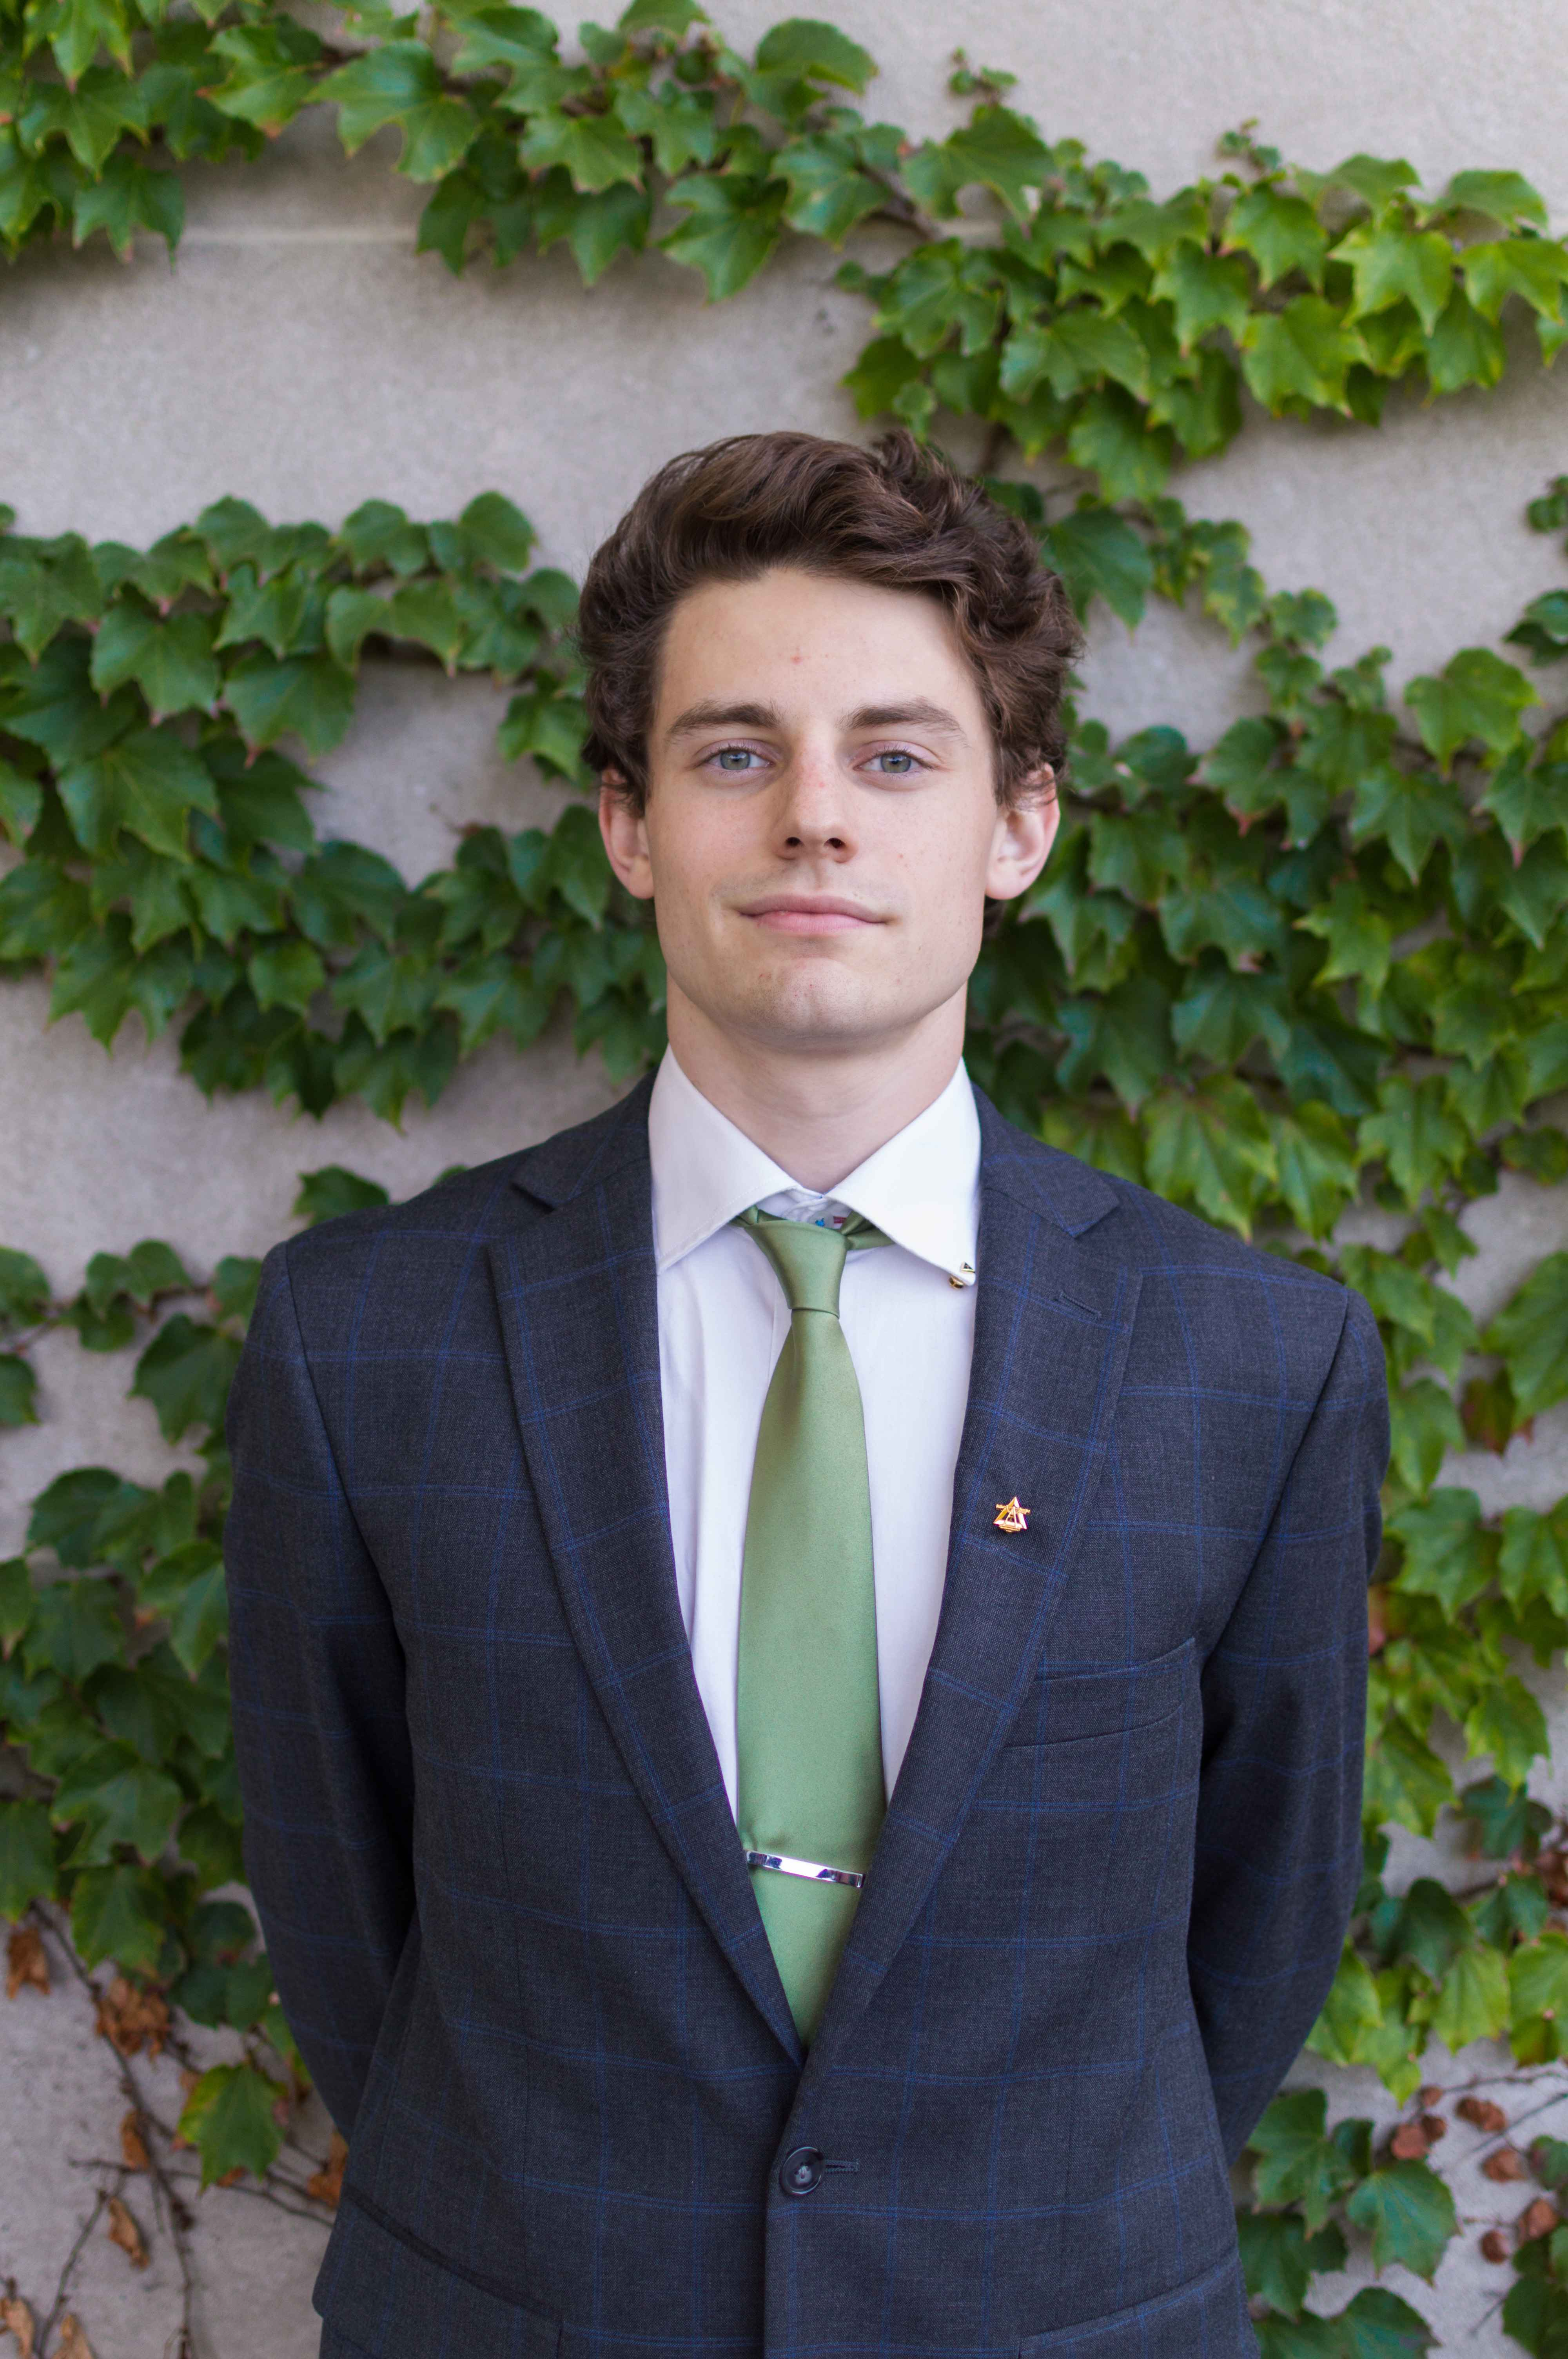
\includegraphics[scale=0.02]{./Hallsby_Karl.jpg}
        \caption*{Karl Hallsby}
        \label{fig:Karl_Hallsby}
      \end{figure}
      B.S. Computer Engineering \\
      M.S. Computer Engineering
    \end{column}
  \end{columns}
\end{frame}

\section{What is RISC-V?}\label{sec:What_is_RISC-V}
\begin{frame}
  \frametitle{\nameref{sec:What_is_RISC-V}}
  \begin{itemize}
  	\item RISC-V is a new, open-source, RISC ISA standard
  	\item Provides several different feature set levels (32-bit, 64-bit, integer, floating point, etc.)
  	\item Suitable for use in applications ranging from microcontrollers to supercomputers
  	\item Goal\textrightarrow become the industry standard ISA
  \end{itemize}
  
  \cite{FireSimTalk1}
%  
\end{frame}

\section{What is Chipyard?}\label{sec:What_is_Chipyard}
% Image of silicon they've taped out using Chipyard and its associated tools
\begin{frame}
  \frametitle{\nameref{sec:What_is_Chipyard}}
\end{frame}

\section{What We Did}\label{sec:What_We_Did}
\begin{frame}
  \frametitle{What We Did}
\end{frame}

\section{What We Learned}\label{sec:What_We_Learned}
\begin{frame}
  \frametitle{\nameref{sec:What_We_Learned}}
  % TODO: Include the challenges we faced while working on this project here
  
\end{frame}

\section{Next Steps}\label{sec:Next_Steps}
\subsection{Educational Laboratory Work}\label{subsec:Educational_Lab_Work}
\begin{frame}
  \frametitle{\nameref{subsec:Educational_Lab_Work}}
\end{frame}

\subsection{Further Research Work}\label{subsec:Further_Research_Work}
\begin{frame}
  \frametitle{\nameref{subsec:Further_Research_Work}}
  \begin{itemize}
  	\item Increase compatability with components on Arty FPGA board
  	\item GPIO, Ethernet, LEDs, Switches, external devices, etc.
  	\item Design and integrate GPIO device that will assist with debugging (single-step bus cycle, display current memory address, program counter, register contents)
  	\item Investigate VLSI Design flow in Chipyard
  	
  \end{itemize}
\end{frame}

\section{Conclusion/Deliverables}\label{sec:Conclusion_Deliverables}
% The Book and our documentation
\begin{frame}
  \frametitle{\nameref{sec:Conclusion_Deliverables}}
\end{frame}

\section{Demonstration}\label{sec:Demonstration}
\begin{frame}
  \frametitle{\nameref{sec:Demonstration}}
\end{frame}

\begin{frame}
  \frametitle{References}

  \printbibliography[heading=bibintoc]{}
\end{frame}

\end{document}

%%% Local Variables:
%%% mode: latex
%%% TeX-master: t
%%% End:
